%!TEX root = ../dokumentation.tex
% -------------------------------
\chapter{Design} % ~4–5 pages, ~1600–2000 words
% -------------------------------
\label{chap:design}


% \section{Requirements}
% Aus Kapitel 1 breiter ausgeführt, ASTRA_sim bezogen, usability etc.
ASTRA-Sims versions allow differentiated research, depending on goals and configurations.
The to be developed \ac{UI} should make one suitable version compatible with the usage of novice users such as \ac{HPE} presales.
Best practices of \ac{UI}/\ac{UX} design should be considered while using an existing version of \ac{ASTRA-Sim}. To optimize inputs and outputs of it, knowledge of \ac{DML} needs to be known and referenced.



\section{Requirements Analysis}
% zb viele excel files = Graphs idk -> konkret darauf eingehen was gebraucht wird

% Persona
To understand the broad description of \textit{\ac{HPE} Presales} for the \ac{HPC} infrastructure direction, a simple persona was created. 
As there was no data about this target group available, is the persona based on 1. expert knowledge gained by interviews with employees with more background knowledge and 2. assumptions about non-experts in the \ac{DML} field. 
The website will be designed based on this persona and with user tests later on adjusted.

The designed persona is ``Angelina B. Smith''. She is a 34 year old employee in the \ac{HPC} department.
More detailed information can be found in the appendix~\ref{appendix:B}, here the most relevant information gets presented.
She got a bachelors degree in business informatics and has been in her role as a ``Presales Specialist for AI & HPC Infrastructure'' for 2 years.
Her goals are to convince customers with infrastructure proposals that suit their expectations, communicate the complex technical concepts clearly and build trust with the customers. At the same time she has the fear to overwhelm customers and not understanding new tools. Tools she does use currently are Excel and PowerPoint, and she likes working remotely and in the office, with her laptop but also smartphone.
She has an example knowledge of \ac{IT} infrastructure and network topologies, but no deep knowledge of simulation tools or \ac{DML}.

Based on the persona perspective the primary identified aspects of inputs are:
\begin{itemize}
  \item \textit{Understandable}: The user needs to understand easily what the input means that they are entering
  \item \textit{Easily Reproducible}: A user should be able to reapply known experiments and modify them for easy comparison. This is important for the use case and a feature the \ac{CLI} based version of ASTRA-Sim includes.
  \item \textit{Accessible}: The inputs should be easily identifiable as clickable and the values should be easily inputable. Ideally would be if the user gets an implicit guidance through the inputs even if they have not much expertise.
\end{itemize}

And the outputs should be:
\begin{itemize}
  \item \textit{Understandable}: The user should be able to understand the results at the first view, without detailed prior knowledge on the topic and on the visualizations. This is especially important as visualizations might be used for discussions with customer, which might not have a background in the \ac{DML} field.
  \item \textit{Easily Exportable}: Similarly to inputs should outputs be able to be exportable to include them in presentations or process them manually in the current workflow with Excel files.
\end{itemize}

% TODO hier kann ich noch mehr schrieben und mich noch mehr auf kapitel 2 beziehen


% \section{Technologies and Architecture}
\section{Technologies}
The to be developed \ac{UI} will be part of a full stack web application. The choices of technology are based in two ways. One, to fulfill \ac{UI} best practices and two, be suitable for the extent of the project.

The interior design of the website was made with Figma. That is a tool that supports early detailed wireframes, which are necessary for early user feedback and evaluation.
The frontend implementation includes a TypeScript React framework based on Vite and node.js. % TODO check if that makes sense
This setup was chosen as it supports component based development with grommet and type checking. For a consistent experience within the product but also next to existing \ac{HPE} websites, the components are based on Grommet. That provides pre-configured components all reflecting the branding, and look and feel of \ac{HPE} webpages.

The backend is a Flask server based on Python. That allowed a lightweight \ac{API}, which purposes it is to be the pipeline between the \ac{UI} and \ac{ASTRA-Sim}. Pythons right library availability also allowed for plots of \ac{CSV} outputs to be created and send to the frontend. 

To complete the setup, the frontend and backend are organized via docker containers. This allows including different versions of \ac{ASTRA-Sim} in the future with minimal effort.

% grommet = branding
% flask API = einfacher astra sim zugang
% react = wegen grommet
% TS = wegen data consistency ( evtl braucht astra sim des halt wegen viele inputs und so)
% python = vorliegende scripte, simple API
% Docker = Container vs keine = easy ASTRA-sim deployment (installationen dependencies etc), Separation of concerns
% Figma = usability pretesting, early feedback & user tests

% TODO was fehlt: warum wizard & dass spliten zwischen advanced und net bzw usage of default parameters
% The choice to use a wizard


\section{UI/UX Design Process}
% Wireframes, heuristics
% Immer Bezug auf Kapitel 2.3 nehmen! Wegen wissenschaft und so
% 1. Overview (Branding & Wizard)
% 2. ASTRA-sim Inputs (analyse (prio, thema weil falsch), beispiel & default werte (tablellen), UI entscheidungen Input type)
% 3. ASTRA-sim Outputs (analyse, visualisierungs  möglichkeiten, evtl data science block für weitere extensions denn das würde python legimatisieren)
% 4. Extended Features: Import & export, History
% 5. Umsetzung: Wireframe first idea what was bad, next idea, what was bad now idea what is bad oder so

% \begin{figure}[H]
%     \centering
%     \includegraphics[width=0.8\textwidth]{figures/cli_vs_ui_workflow.png}
%     \caption{Concept diagram: CLI workflow vs UI workflow}
% \end{figure}

There were two main approaches to design the general \ac{UI}.
The first was to use a multistep form, called a wizard. In it the user gets guided through the necessary input parameters and gets support for understanding what they mean. This has the advantage that user exactly knows what is expected from them. They cannot forget to enter specific information and the inputs are easily reproducible. Also, compared to a single page form, the user gets less overwhelmed by the amount and diversity of available parameters.
The alternative idea was a natural language interface in which the user can enter questions about specific \ac{DML} configurations and gets general results. This idea was inspired by AskCricinfo, a \ac{NLP} based web-based information retrieval system for cricket games\footnote{https://www.espncricinfo.com/ask}.
That brings the advantage of giving the user a high level of accessibility and an easy way of learning.

Ultimately, it was decided against the \ac{NLP} based idea as it does not give the user enough guidance for the usage of the tool and is not suitable for the requirement of not overloading a users' cognitive load, as it requires a high amount of self thinking and knowledge to use such a tool in a complex area like \ac{DML}. A wizard was chosen with the potential opening to an additional \ac{NLP} input field in the future.

The design process was developed iteratively. First, a general draft for the page navigation was proposed and evaluated. Then more specific wireframes have been designed and were iteratively improved in two iterations.
The feedback in both rounds was collected in a free format, which allowed feedback givers not to feel limited to certain aspects but of course is not scientifically holdable.
The first round of feedback was provided by employees in the \ac{HPE} Labs who can be considered familiar or experts with \ac{ASTRA-Sim} and know how to use it. The second round was done in the environment of an intern fair in which \ac{US} \ac{HPE} employees were able to get informed about current projects and are able to give early feedback. % TODO introduce the US acronym before because it is ugly here

The first draft of the general website can be found in figure~\ref{fig:wire-1}. It shows the navigation next to how one page of the wizard could have been structured.

\begin{figure}[h]
    \centering
    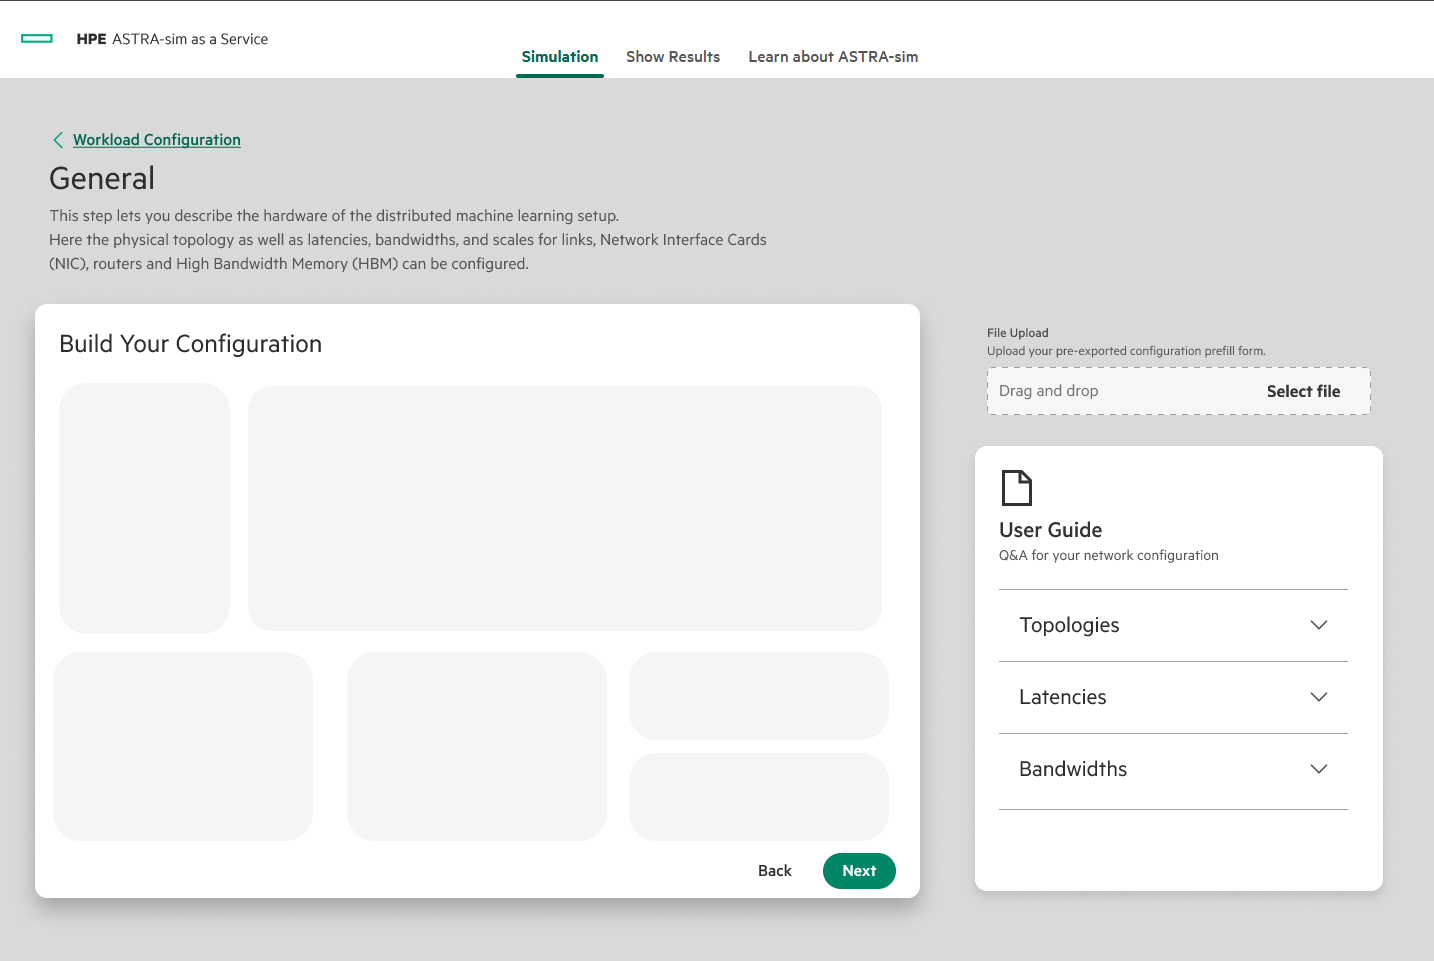
\includegraphics[width=0.75\textwidth]{first-wireframe.png}
    \caption{General Wireframe v1.0}
    \label{fig:wire-1}
\end{figure}

This page features roughly five components that have to be mentioned. A header, a headline, the input fields, a file upload and a user guide. 
The header that is displayed holds three tabs, being the simulation configuration, the results and an additional training page for getting more background information. This reflects the two main purposes the page serves to simplify usage of \ac{ASTRA-Sim}, with simplifying inputs, and outputs and additionally providing direct access dor guidance for non-experts. \\
The headline on top shows which step of the wizard the user currently is at. It also leaves room for a short explanation and a button to the previous page, because users might expect that in the top left corner.
The input fields are individual by what page the user is at and which inputs they gave before. In this wireframe version this page is located on the left, implicitly getting attention before the last two components but not getting the full focus.
The file input was decided to put on every wizard page to allow uploads for every layer directly which makes it easy to directly visualize and modify inputs. \\
The user guide, located on the right down corner was supposed to contain descriptions of the input fields for the user to click if necessary.

For a more specific view the network page of this base is displayed in figure~\ref{fig:wire-2}. It includes parameters for the number of dimensions, possible topologies for each dimension and configurations for links like their number, bandwidth and latency. That way it displays \acp{ASTRA-Sim}' inputs for the network layer excluding \ac{HBM} details.

\begin{figure}[h]
    \centering
    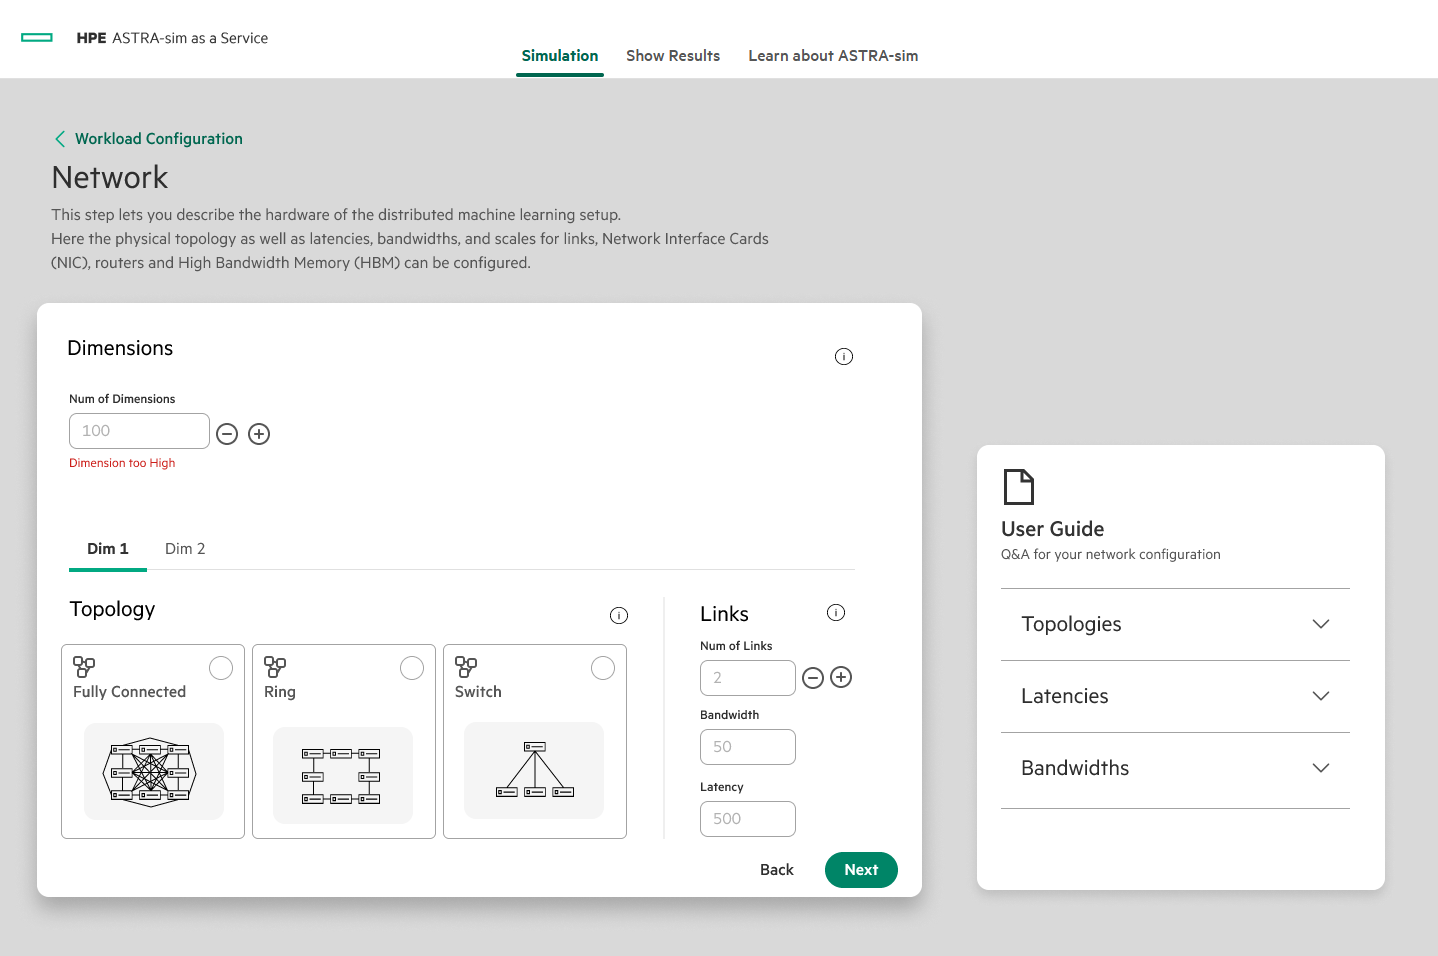
\includegraphics[width=0.75\textwidth]{first-wireframe-network.png}
    \caption{Specific Wireframe Network v1.0}
    \label{fig:wire-2}
\end{figure}

This setup includes help for the user for example by providing pictures of the available topologies and a dynamic way of adding in dimensions. Additionally, it includes an information button for every input subcategory, that opens a descriptive popup. That aims at increasing flexibility between experts and novice users by subtilely supporting novices learn process. 

Problems with that setup can also be seen at first glance. Fitting all inputs of one layer of \ac{ASTRA-Sim} is not possible with the space available in the chosen wizard layout.
Also, the connection between the headline and descriptive text to the wizard content as well as the connection between the wizard and the user guide is not intuitively noticeable. One further critic point is that the link inputs are located to the right of the topology inputs, making them easily overlooked, because they are not below the topologies where the user would expect the to be.

While this initial draft has the strength of supporting users' necessity of help and gives them direct access to many features it lacks one specific but very important criteria, being to not overload the users' cognitive load.
For example with adding the file upload field on the same page as the inputs, the user could already be confused and challenged by the system. It might not be easy to understand that the file upload is optional, and the user might be confused by the structural logic of needing to click through all pages to upload specific files, a task that is repetitive and not to the point. \\
Therefore, if evaluated by the $69$ rules of \ac{UI} design, as presented in chapter~\ref{chap:literature}, it actively disregards the rules $1$, $3$, $4$ of the recognition category, rule $2$ of flexibility, rule $2$ of consistency, and rule $1$ of navigation.

% gehe hier vorallem daurauf ein wie die logische sequenz des wizards vereinfacht wurde von der dummen sequenz von astrasim zu einer sinnvollen, user spezifischen
To improve this design two steps were taken. First, all inputs were revised and newly categorized and second, the general page structure was restructured. The first step was necessary, because the full set of $25$ input parameters is rather too much for the user and therefore only the most influential and target group specific parameters should be asked for. The second step naturally follows from presented challenges to reduce navigation complexity and provide a more accessible navigation. 

The full classification of inputs can be found in the appendix~\ref{appendix:inputs}.
The $22$ inputs of \ac{ASTRA-Sim} plus additional three parameters that are included within the \texttt{workload.txt} file were collected and prioritized. This priority was estimated based on how huge the influence of certain parameters is compared to others. \\
Therefore, parameters such as \textit{topologies per dimension} were considered important, because physical topologies can make huge differences in \ac{DML} setups and are important for the user to configure, while inputs such as \textit{preferred dataset splits} are considered rather unimportant as it is only small influential factor, that can also be easily estimated by default factors of other parameters such as the provided workload. \\
Next, it was identified which inputs could be made more accessible for the user with only little prior knowledge. These include the workload parameters, which are usually depending on which specific model should be trained.
If we assume the target user does not know specifics such as the workload, they could for example choose one prior configured model type whose parameters can be estimated.

Next, the identified parameters were newly categoriesed, as the \acp{ASTRA-Sim} mapping is in parts misleading. \\
For example is \ac{HBM} misleading to include in the network section, as it functions as an accelerator, not a primary part of the network. \\
Three new categories were identified. First, the network, in itself separated into general network settings and link specifics; workloads and the associated collectives and additional accelerators. 
For a logical sequence that feels natural for the user the sequence in figure~\ref{fig:wizard-flow} gets proposed.

\begin{figure}[h]
    \centering
    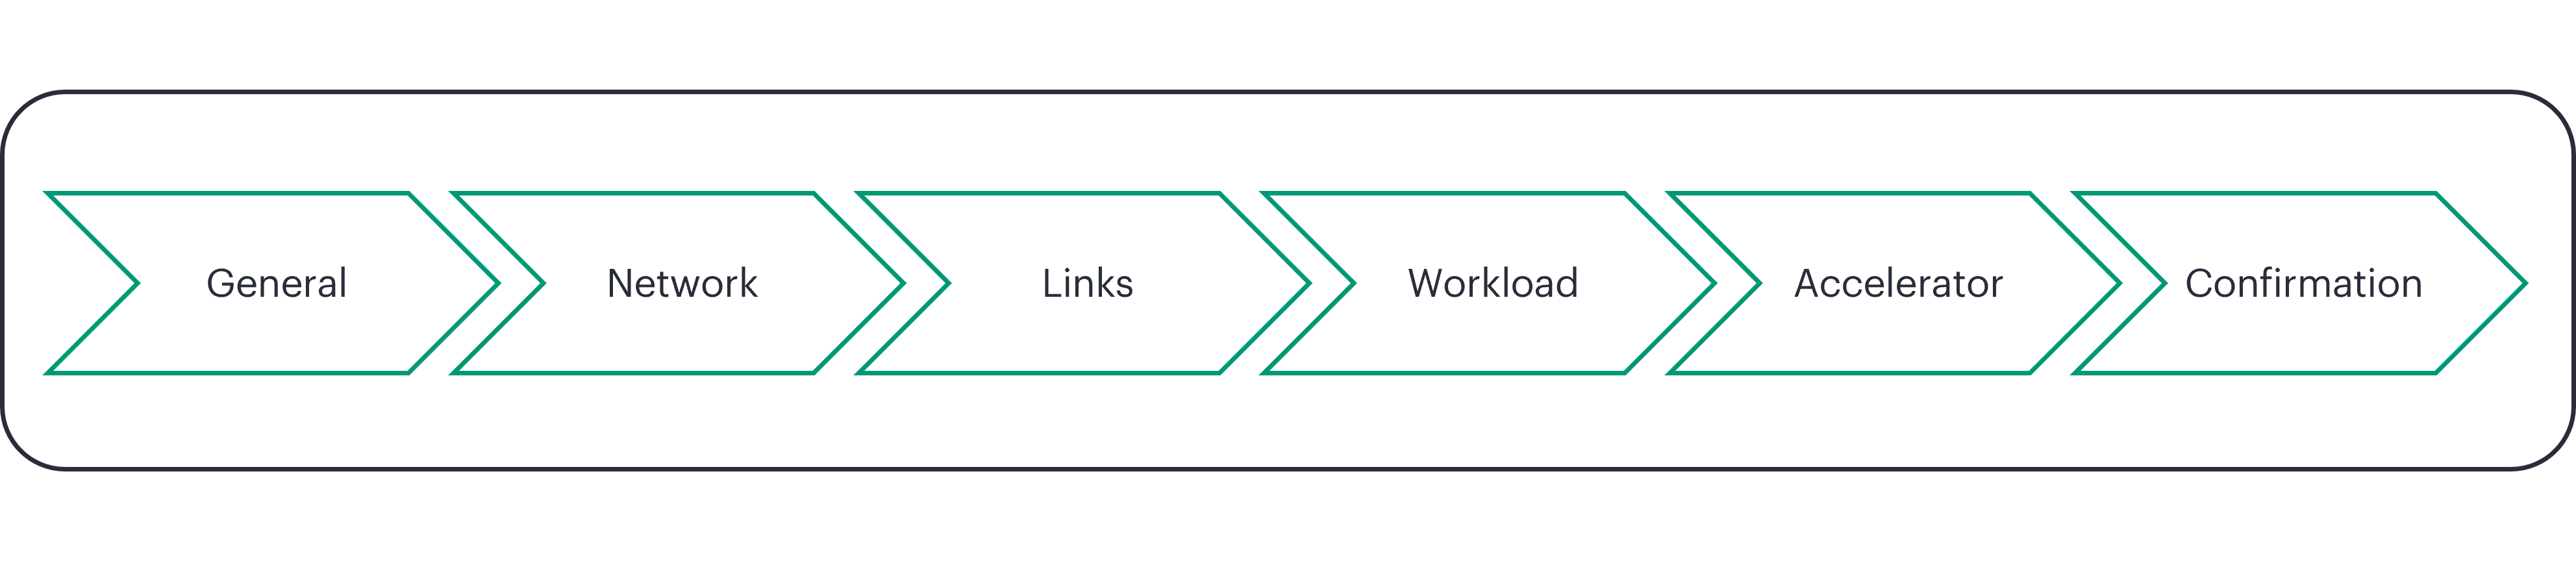
\includegraphics[width=1\textwidth]{wizard-flow-alternative.png}
    \caption{Wizard Page Flow}
    \label{fig:wizard-flow}
\end{figure}

The user gets to choose general information such as the workload model or a configuration of the history of their previously simulated runs.
The network category is the first thematically page as the users main knowledge lays in that field. This aims at not overwhelming the user as they feel familiar with inputs. That makes the first rule of the recognition category apply.
Next following is the category of links, as that is a subcategory of the network and therefore connects seamlessly. \\
Next, the workload gets specified. That choice was made, because this page mainly focusses on specifying logical topologies. Therefore, it makes sense to put it as closely as possible to the physical topology to make the navigation back to the physical topology to check the difference as easily as possible. \\
Then, the accelerator is added to give it the feel of configuring additional hardware to make the \ac{DML} training process faster. 
Lastly, a wizard page that sums up all inputs was added too. That is a wizard best practice that provides an easy input confirmation to reduce user caused simulation miscalculations. 

Figure \ref{fig:wire-3} shows the final wireframe of a wizard page on the same example, which is the network category. 

\begin{figure}[h]
    \centering
    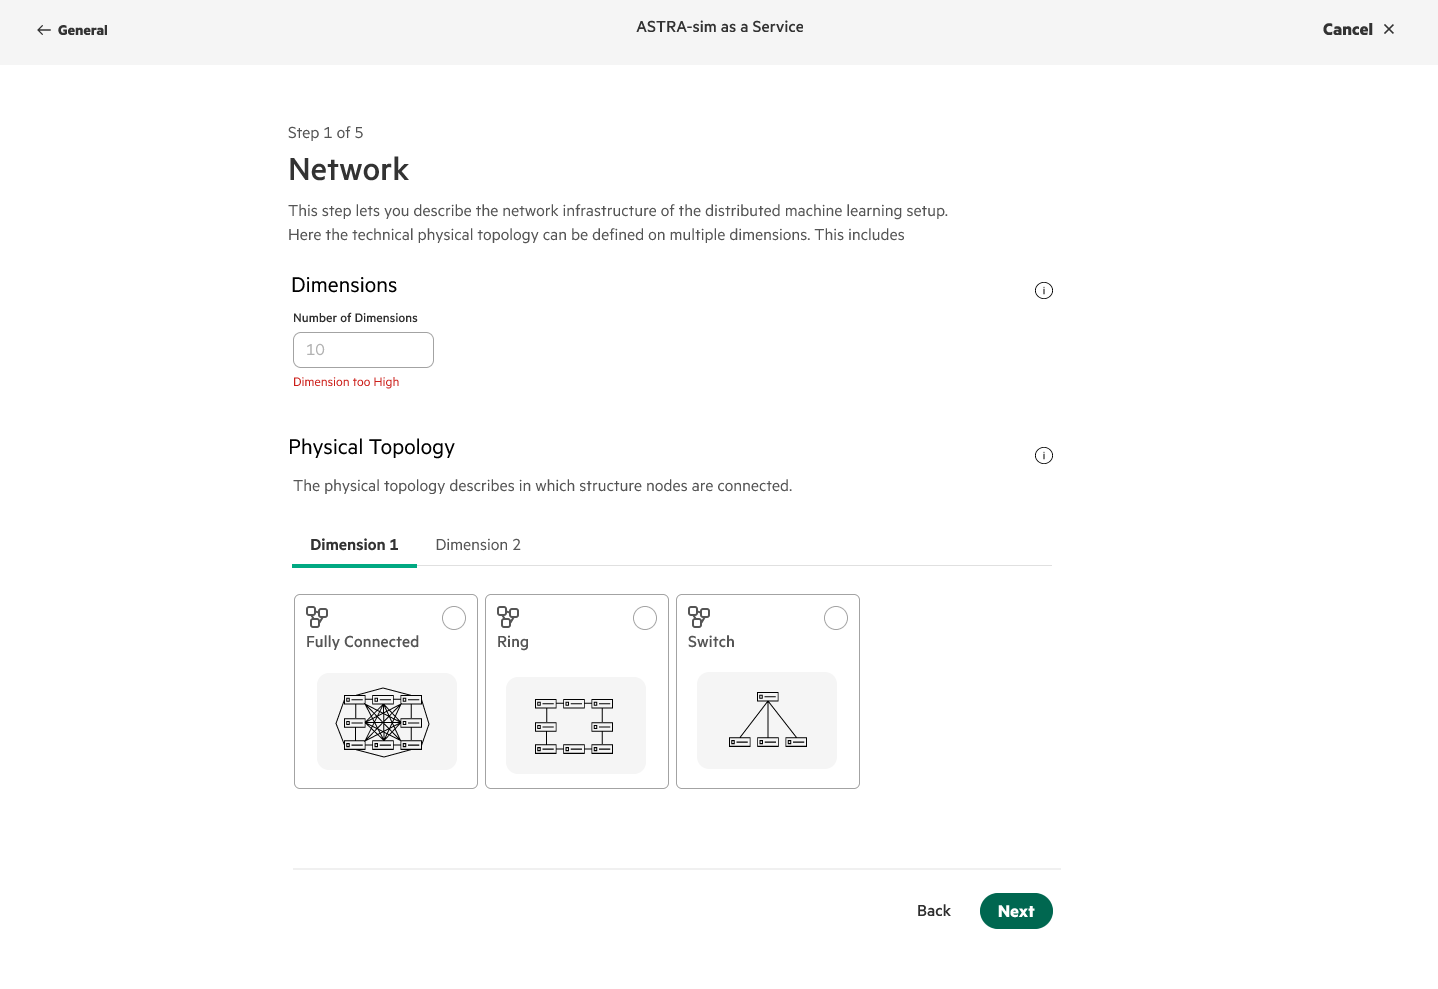
\includegraphics[width=0.75\textwidth]{later-wireframe-network.png}
    \caption{Specific Wireframe Network v2.0}
    \label{fig:wire-3}
\end{figure}

The first improvement made was to change the subpage wizard to a full-page wizard. Not only does this comply with \ac{HPE} internal branding guidelines, but it also makes the user focus all their attention to the most important steps. That solves the issue of rule $4$ of the recognition being violated before. \\
Other details were changed, like a specific feedback if users break rules set by the \ac{UI}. That way, for every parameter, a set of allowed parameters was configured to guide the user and make it hard for them to input unuseful configurations.
For instance, the upper limit for configurable dimensions was $5$, as dimensions up to $3$ are expected, but the user should get a little upper flexibility for more complex setups. Higher dimensions do not make sense for a realistic simulation and can potentially overwhelm the user, as with every added dimension, a linear increasing amount of additional input fields get added. \\
Another improvement for this setup is, that all wizards inputs are arranged under each other, never next to each other, except for choices of one input. That ensures predictability of the wizard and an understanding for the user, which is important for the rules of the category navigation.

In one last iteration, last informal and unstructured feedback was included to update to a final implementation. Figure~\ref{fig:wire-4} shows the final wireframe of the network page.

\begin{figure}[h]
    \centering
    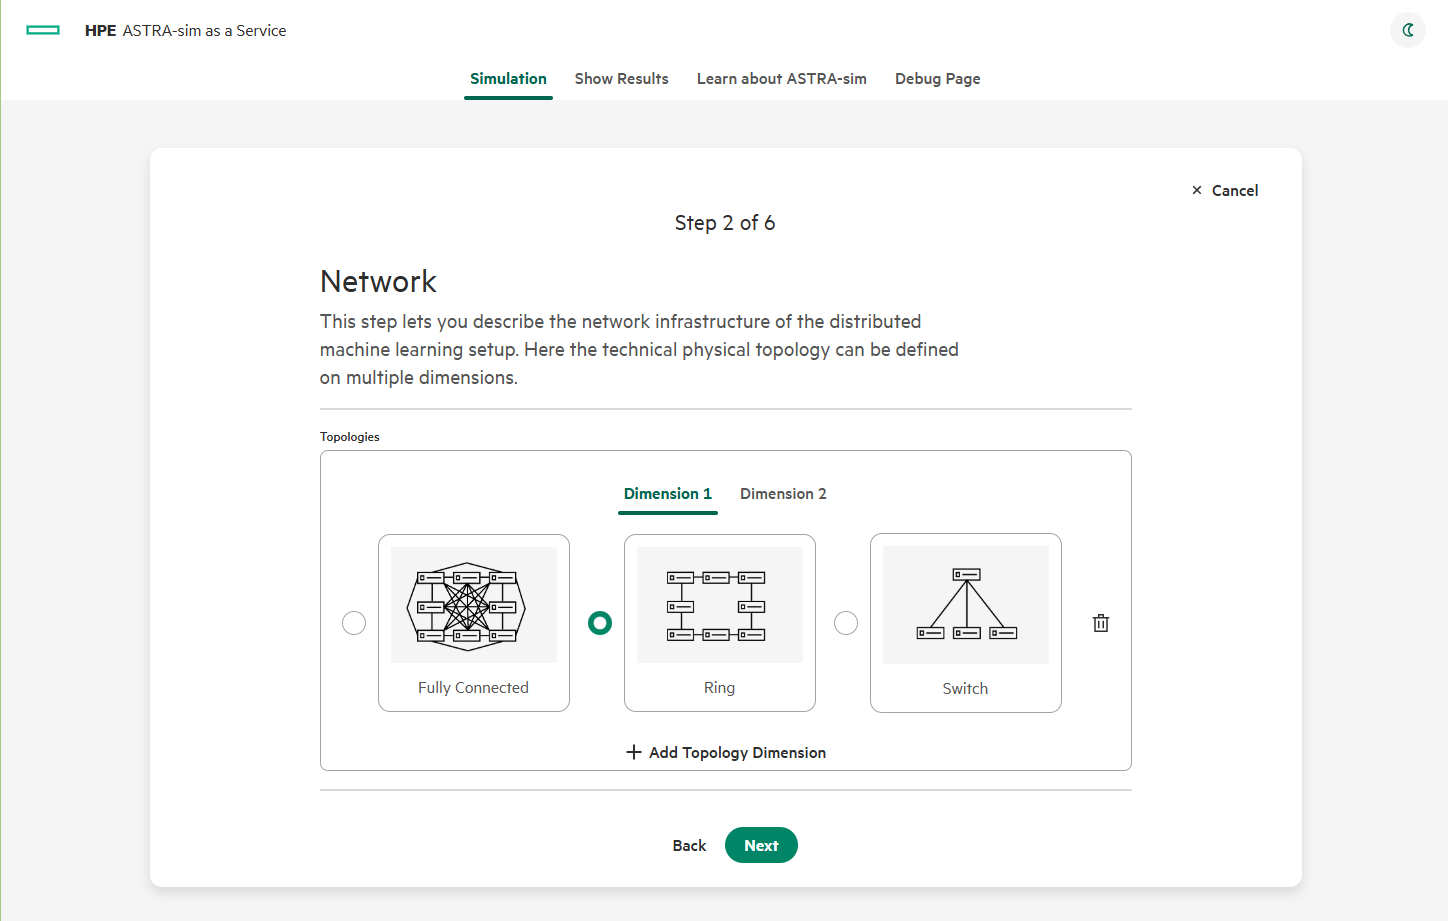
\includegraphics[width=0.75\textwidth]{implementation-network.png}
    \caption{Final Wireframe Network Page}
    \label{fig:wire-4}
\end{figure}

One major difference to the previous designed wizard is that this one is not full page again. That design was chosen to awake the feeling that the wizard is integrated into the whole page and less an additional thing. In the end, this is the part where users might spend the most time.
Another difference is, that the count of dimensions was integrated into the choice of physical topology. That way, the association between the count of dimensions and their actual existence gets more obvious for the user. 
Also, actual colors differentiate from the previous configurations, suiting current corporate branding suggestions. 
% TODO die i für information fehlen!!!



% Mentionable recommendations for instance also include that systems should enable users to easily recognize user functions (recognition, rule 3), it should ensure consistency in appearance (consistency, rule 1), it may concentrate the information mainly in the center of the screen (visual, rule 2), and it should provide the options and information in a logical sequence (navigation, rule 1). Further relevant rules are presented in chapter \ref{chap:design}.


% \begin{figure}[H]
%     \centering
%     \begin{subfigure}[b]{0.48\textwidth}
%         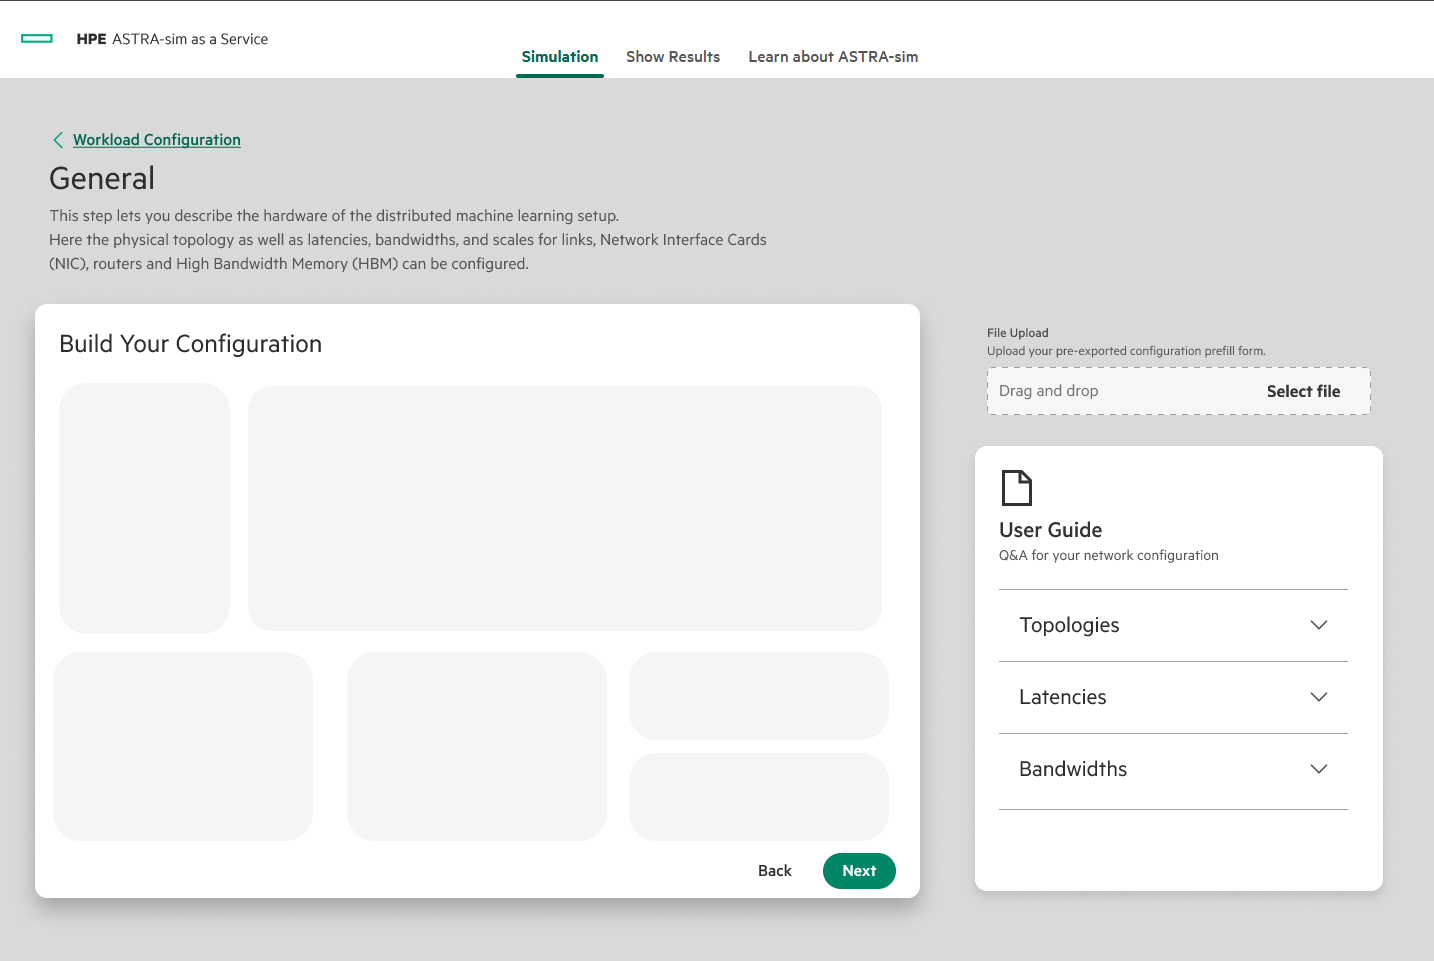
\includegraphics[width=\textwidth]{first-wireframe.png}
%         \caption{First General Wireframe}
%         \label{fig:wire-1}
%     \end{subfigure}
%     \hfill
%     \begin{subfigure}[b]{0.48\textwidth}
%         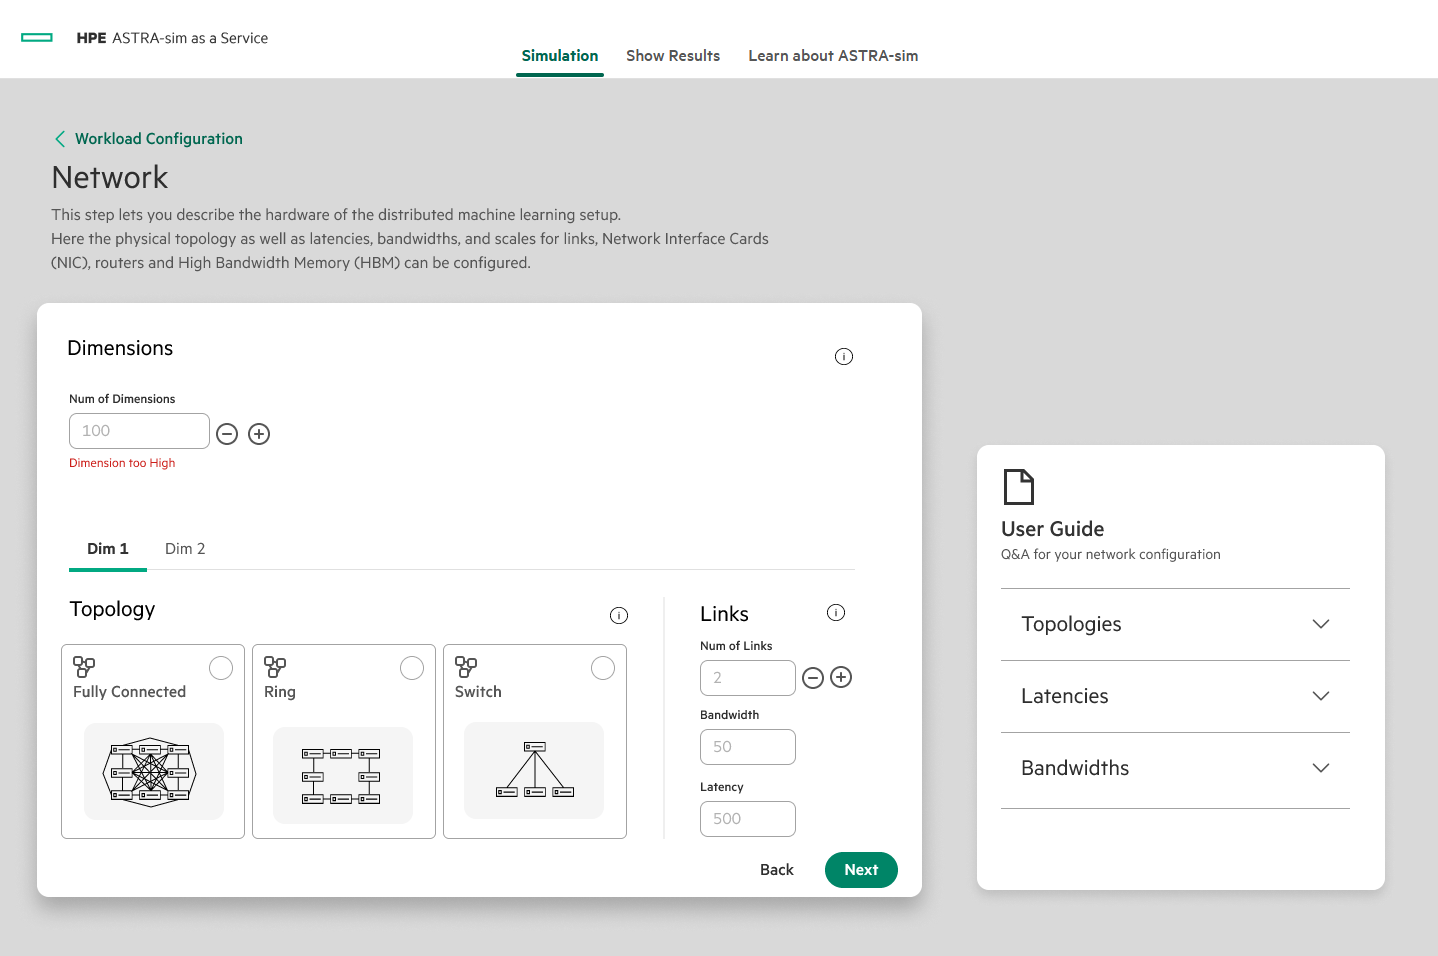
\includegraphics[width=\textwidth]{first-wireframe-network.png}
%         \caption{First Network Wireframe}
%         \label{fig:wire-2}
%     \end{subfigure}

%     \caption{General Structure Overviews}
% \end{figure}


% \begin{figure}[H]
%     \centering
%     \begin{subfigure}[b]{0.48\textwidth}
%         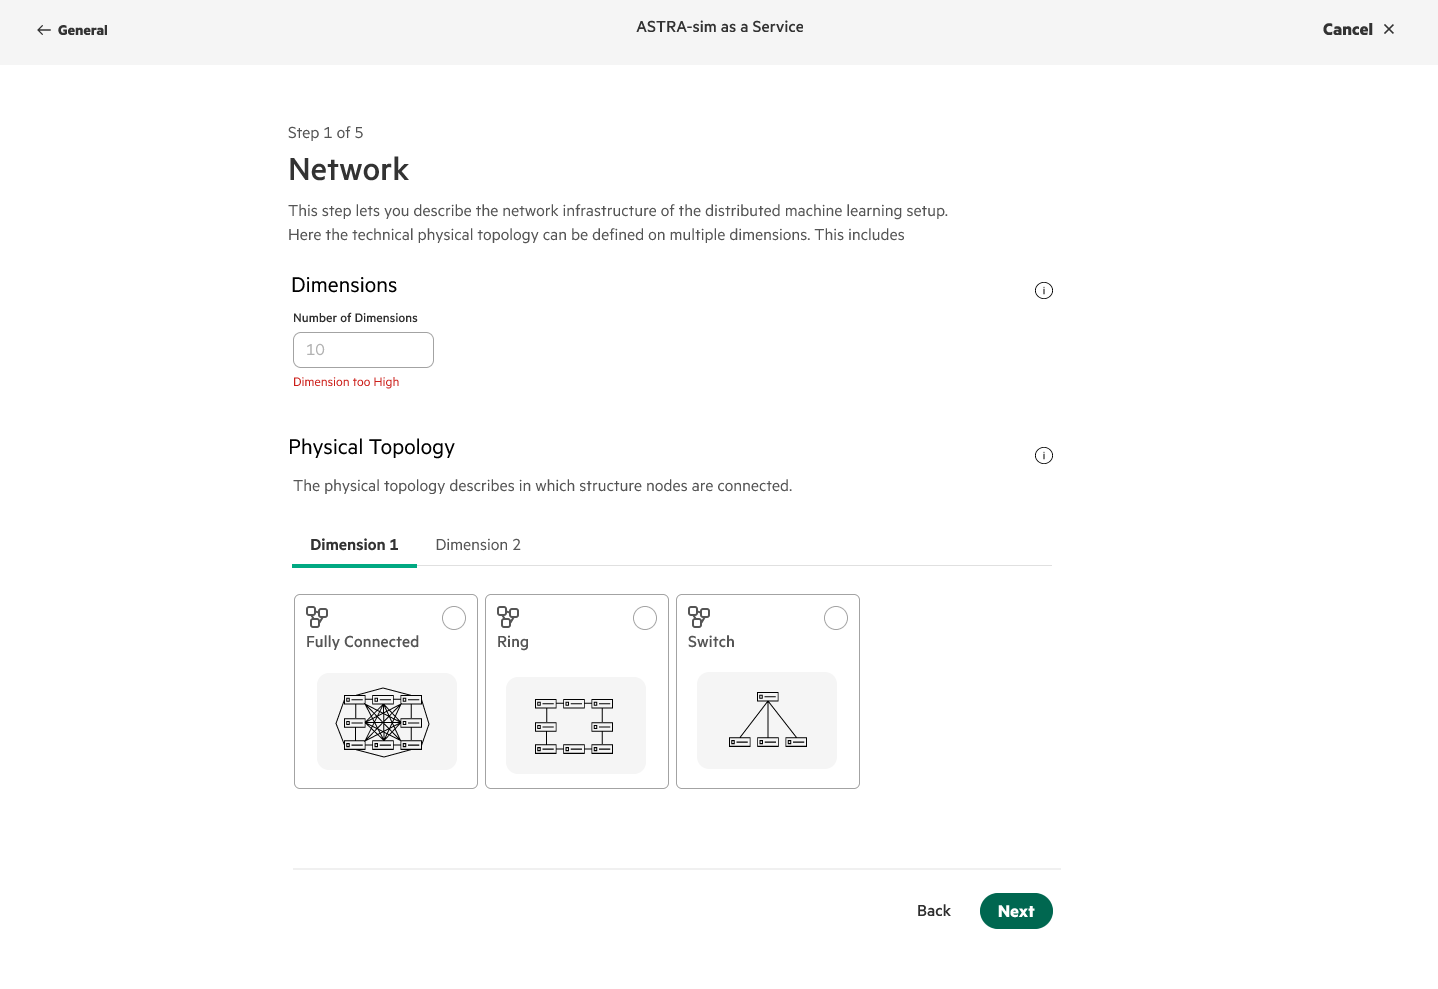
\includegraphics[width=\textwidth]{later-wireframe-network.png}
%         \caption{Adjusted Network Wireframe}
%         \label{fig:wire-3}
%     \end{subfigure}
%     \hfill
%     \begin{subfigure}[b]{0.48\textwidth}
%         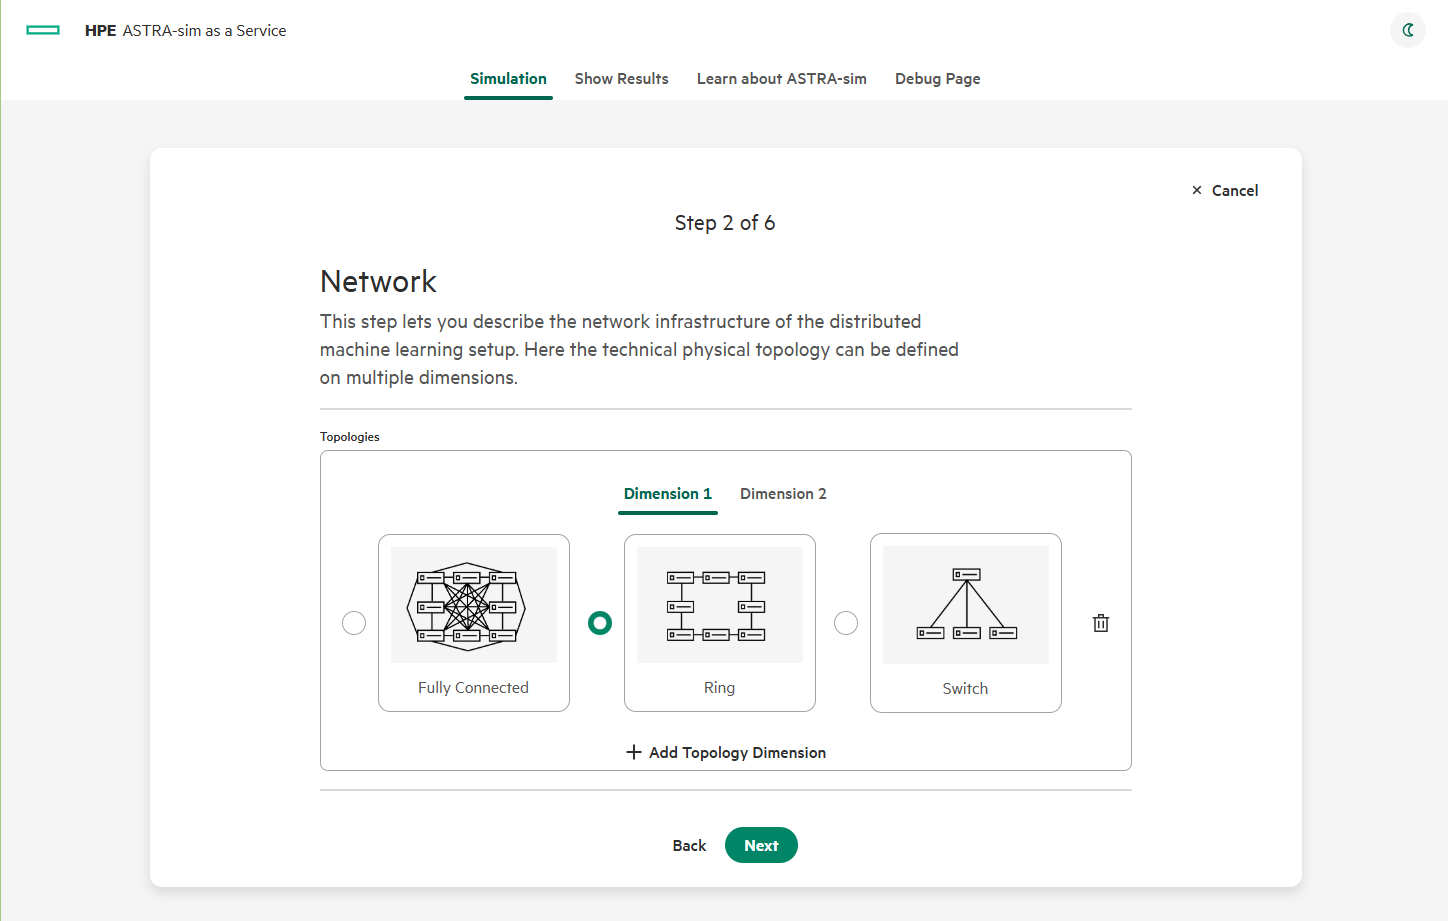
\includegraphics[width=\textwidth]{implementation-network.png}
%         \caption{Final Network Page Implementation}
%         \label{fig:wire-4}
%     \end{subfigure}
%        \caption{General Structure Overviews}
% \end{figure}